\documentclass[12pt,a4paper]{jbook}

\usepackage{mm-thesis}
\usepackage[dvipdfmx]{graphicx}
\usepackage{latexsym}
\usepackage{amsmath}
\usepackage{amsthm}
\usepackage{amsfonts}
\usepackage{cite}
\usepackage{comment}

\thesis{\master}
\title{webの汎用的解析に向けた時相論理の表現による形式検証}
\author{島本 隼人}
\supervisor{藤原 融 教授}
\deadline{2017年2月15日}

\documentclass[12pt,a4paper]{jbook}
\usepackage{mm-thesis}
\usepackage[dvipdfmx]{graphicx}
\usepackage{cite}
\usepackage{comment}
\usepackage{docmute}
\usepackage{color}
%\usepackage{amsmath}
%\usepackage{amsthm}
%\usepackage{amsfonts}

\begin{document}

ウェブの発展に伴い個人情報を取り扱いが増加しているため、その通信の安全性が重要となっている。
一方で、ウェブの構造は一般的なシステムと比べ複雑となっている。
このようなシステムに対しては、適当な入力を与えて実際の動作を確認するといった従来の手法による安全性解析は時間がかかり、また、漏れが生じる可能性が高く現実的ではない。
そこで近年は、システムの仕様と安全性要件を抽象化したセキュリティモデルを用いた形式手法による解析が盛んにおこなわれている。
形式手法を用いることで、漏れのない自動化した検査を実現できる。
しかし、形式手法の入力となるセキュリティモデルの記述が不十分である場合、解析結果に潜在的な危険性が存在する場合がある。
このような背景から、セキュリティモデルの検討が重要である。

本研究では、既存のウェブセキュリティモデルにおいて包括されている時相論理が不十分であることに注目する。
セキュリティモデルにおいて、時相論理はシステムの状態変化を表現する能力を持ち、システムの正確な安全性解析には不可欠な項目である。
しかし、現状の既存のモデルでの時相論理では、ある一つの通信によるウェブの状態変化しか捉えることができず、二つ以上の通信が互いに及ぼす影響性を考えることができない。
これは、捉えることのできる状態の変化が対となるリクエストとレスポンス間に限られているためである。
この理由としては、既存のウェブセキュリティモデルで利用しているAlloyという形式手法ツールが時相論理に元々対応していないことが挙げられる。
時相論理では「次の状態では~」といった時系列順を用いた論理が用いられるため、Alloyを利用する上ではその時系列を捉えられるよう独自の記述法が必要となる。
\color{red}
%既存文:しかし、グラフを用いた直観的な出力結果を得られる点や、拡張を前提とした基礎研究が確立されており、これを利用した後続の研究も進められている点を考え、Alloyを用いたモデルの拡張が求められる。
%comment:akhaweのモデルを拡張することの信頼性について掘り下げる
しかし、ウェブに対して形式手法を用いる研究ではAlloyを用いた先行研究が確立されており、かつ、その先行研究を応用した研究も数多く存在するため、その先行研究の信頼性は確かなものである。
これに加え、Alloyを使用することでグラフを用いた直感的な出力結果を得ることができ、安全性解析をより効率的に進めることができるため、Alloyを用いたモデルの既存モデルの拡張が求められる。
\color{black}
このような背景から、様々なウェブ要素に対して汎用性のある、Alloyでの時相論理の記述法を作成する。
この時相論理を実現する方針は、対象の要素の各状態を保存するインスタンスのフォーマットを定め、その時系列を考えるために必要となる「最初の状態」と「ある状態の次状態」を判定する述語を作成するというものである。
この述語を利用することで状態の時系列変化を捉えられるため、前もって対象のウェブの要素が時間変化によってどのような状態変化が発生しうるかを仕様書から明らかにしておき、時系列順で前後に並ぶ状態間に対する論理式として記述することで時相論理を実現できる。

また上記の時相論理の設計に加え、この記述法を用いてキャッシュを記述した、新たなウェブセキュリティモデルを作成し評価を行う。
\\(ここから事例研究について書きます)

\end{document}


\begin{document}

\coverpage
\tableofcontents
\listoffigures
\listoftables
\body

\documentclass[12pt,a4paper]{jbook}
\usepackage{mm-thesis}
\usepackage[dvipdfmx]{graphicx}
\usepackage{cite}
\usepackage{comment}
\usepackage{docmute}
\usepackage{color}
%\usepackage{amsmath}
%\usepackage{amsthm}
%\usepackage{amsfonts}

\begin{document}

\chapter{はじめに}
近年、個人情報をウェブ上でやり取りする機会が増えている。
これは、ウェブを利用できる携帯端末が普及したことにより、ウェブ上のサービスが充実してきたことに起因する。
例えば、以前では窓口やATMによって振り込みの手続きを行っていたが、現在ではネットバンキングを利用することでどこからでも簡単に手続きを行うことができる。
したがって、通信内容に含まれる個人情報の増加によりウェブの安全性が極めて重要となっている。
一方で、システムの安全性を検査する際には、システムに適当な入力を与え動作をシミュレーションする方法が一般的に採用される。
しかし、企業等で運用されるシステムに比べウェブの構造は非常に複雑である。
これは、ウェブの運用開始からこれまでにあらゆる拡張が成され、多様な要素が存在するためである。
このように複雑なウェブに対して、適当な入力を与えるシミュレーションでは検査に漏れが生じる可能性が多く、安全性を確実に保証することはできない。

本研究では、ウェブというシステムの安全性を証明する手法として形式手法を利用する。
この手法の利用にはまず、想定される攻撃者の能力、システムの運用環境、満たされるべき安全性要件を論理式を用いて表現したセキュリティモデルを用意する。
形式手法はこのセキュリティモデルを利用し、システムが安全性を満たしているかを数学的に検査する。
これにより漏れのない、より精密な検査が可能になる。
また、この手法の長所として、セキュリティモデルを入力とし専用の解析ツールを用いることで解析を自動化でき、労力を大幅に削減できることが挙げられる。

しかし、前述の通り、ウェブというシステムには様々な要素が含まれており、複雑な構造となっている。
これは、ウェブの目まぐるしい発展により、従来の技術よりも優れた技術が次々に追加されているためである。
このような状況を受けて、これらの膨大な要素の中から現在広く使われている要素を抽出し、それらの要素に注目したウェブセキュリティモデルが提案されている\cite{based-model,cookie-model}。
しかし、これらの既存モデルにおける時相論理が表現できることは、ある一つの通信のやり取りの前後における状態変化のみであり、ある通信が他の通信に及ぼす影響を考えることができない。
本来、ウェブにおいては複数の通信が並列していることが当然であり、この既存モデルでの時相論理の表現力では不十分である。
そもそも、時相論理はシステムの各状態間の関係性を表し、ウェブは時間ごとに状態が刻々と変化するシステムであるため、時相論理による表現は不可欠である。
しかしながら、これらの既存モデル\cite{based-model,cookie-model}は、Alloy Analyzerという形式手法ツールを用いて実装されており、このツールは時間軸を表現するといった機能を持たない。
そのためAlloy上で時相論理を表現するには、ツールの機能に頼らない時相論理の記述法が必要となる。
一方で、既存モデル\cite{based-model}はウェブに対する形式手法の基礎研究として確立されており、またこれを基にしたCookieの研究\cite{cookie-model}を始めとする様々な研究\cite{chaitanya2017formal, bagheri2016practical, chen2015aspire, nelson2013aluminum, somorovsky2011all}が進められているため、これらのモデルを基に拡張を行うことが重要である。
このような背景から本研究の目的は、Alloyを用いて、より正確な安全性検証のために時相論理の拡張を行ったウェブセキュリティモデルの提案である。

また、本研究では上記の時相論理の表現を加えて、時相論理の実装により表現できる要素としてキャッシュに注目している。
キャッシュは広く一般に使われているウェブの構成要素である一方で、既存モデルに含まれていない要素である。
しかし、実際にこれらの要素は近年の成果として報告されている攻撃法\cite{bcpattack}にも利用されており、ウェブの安全性を評価する上で欠かすことのできない概念である。
本研究では、拡張した時相論理を用いてキャッシュの実装も行う。

本論文の構成は以下の通りである。
二章では、形式手法とウェブに関連する知識を述べる。
三章では、本研究の基礎となる既存のウェブセキュリティモデルとその問題点に述べる。
四章では、時相論理を包括したウェブセキュリティモデルを提案する。
五章では、現実に起こりうる事例を取り上げ検証結果を確認することで、提案モデルを評価する。
\end{document}

\chapter{準備}
\section{形式手法}
形式手法とは、これはシステムの安全性を数学的に証明する方法であり、システム設計を手助けする方法の一つである。
一般に産業界で用いられる方法は形式手法とは異なり、作成したシステムに様々な入力を与えて検査する方法である。
この方法では低コストで検査することが可能だが、テストのための入力を人が考えるためシステムに不具合が残る可能性がある。
一方で、形式手法は数学的な証明であるため、そういった不具合を無くすことができる。
また、この手法は専用の検査ツールを利用することで自動化が可能であり、検査に掛かる手間を大幅に減らすことが可能である。

実際にシステム開発に形式手法を利用する際には、以下の四つのステップの手順を行う。
\begin{enumerate}
\item 設計したシステムをセキュリティモデル(\ref{sec:SecurityModel}参照)として表現する。
\item 用意したセキュリティモデルを入力として形式手法ツールを実行し、設計の漏れや仕様上の不具合を検出する。
\item 2.で検出された漏れや不具合を参考にシステムの設計を見直し、その修正をセキュリティモデルに適用する。
\item 2.以降を繰り返す。
\end{enumerate}

\subsection{セキュリティモデル}
\label{sec:SecurityModel}
セキュリティモデルは形式手法における入力にあたり、以下の三要素で構成される。
\begin{itemize}
\item 対象のシステムの構造
\item 脅威モデル
\item 安全性要件
\end{itemize}

\subsection{Alloy Analyzer}
Alloy Analyzerは形式手法による解析ツールの一つである。
検査対象のシステムのセキュリティモデルをAlloyという専用の言語で記述し、これを入力として実行する。
その結果としては二通りの出力を得ることができ、まずは、そのシステムが設計上取りうる状態の例が表示され、これを利用することでシステムが設計者の意図していない挙動を行っていないかを確認でき、設計上の漏れを防ぐことができる。
また、安全性要件を満たさない危険な状態を検索することも可能であり、これによりシステムが設計通りに動作したとしても危険な状態に陥ってしまうような不具合を見つけることができる。

また、Alloy Analyzerが他の形式手法ツールとは異なる点として、実行結果を図として得られるため、より直観的な利用が可能であることが挙げられる。
さらに、Alloy Analyzerは汎用的なJavaを用いて実装されているため、環境の構築はJavaのインストールのみで済み簡単に利用することができる。

\section{時相論理}
時相論理とは、

\subsection{線形時間論理}


\subsection{分岐論理}


\section{キャッシュ}


\subsection{Browser Cache Poisoning攻撃}

\section{中継者}
\subsection{プロキシ}
\subsection{ゲートウェイ}

\section{Hypertext Transfer Protocol}

\section{関連研究}

\documentclass[12pt,a4paper]{jbook}
\usepackage{mm-thesis}
\usepackage[dvipdfmx]{graphicx}
\usepackage{cite}
\usepackage{comment}
\usepackage{docmute}
\usepackage{color}
%\usepackage{amsmath}
%\usepackage{amsthm}
%\usepackage{amsfonts}

\begin{document}

\chapter{既存のウェブセキュリティモデル}
\section{セキュリティモデル}
\label{sec:SecurityModel}
セキュリティモデルは形式手法における入力にあたり、検査対象のシステムを命題論理を用いて表現したものである。
セキュリティモデルに記述する項目は主に以下の三つである。
\begin{itemize}
\item 対象のシステムの構造と動作
\item 脅威モデル(想定される攻撃者の能力)
\item 安全性要件(安全上満たしているべき条件)
\end{itemize}

\section{拡張を想定した汎用モデル}

\section{Cookieを包括するモデル}

\section{既存モデルにおける問題点}

\end{document}

\documentclass[12pt,a4paper]{jbook}
\usepackage{mm-thesis}
\usepackage[dvipdfmx]{graphicx}
\usepackage{cite}
\usepackage{comment}
\usepackage{docmute}
\usepackage{color}
%\usepackage{amsmath}
%\usepackage{amsthm}
%\usepackage{amsfonts}

\begin{document}
\newpage

\chapter{提案モデル}
この章では,\ref{sec:ProposedModel-TemporalLogic}章で述べた記述法の応用例として,キャッシュを実装したウェブセキュリティモデルを提案する。

本研究では基礎モデルで包括されていないウェブの要素としてキャッシュに注目する。
\ref{sec:introduction}章に述べた通りキャッシュを利用する攻撃が数多く存在しており,また,キャッシュは一般的なユーザにも利用されるウェブの構成要素である。
したがって,キャッシュに関連した脆弱性はウェブの利用者に多大な影響を与えるため,ウェブの安全性を解析する上で不可欠な要素である。
本研究では,キャッシュを包括するウェブセキュリティモデルを\ref{sec:ProposedModel-TemporalLogic}章で述べた記述法を用いて実装する。

\section{提案モデルの能力}
\label{sec:ProposedModel-Power}
提案モデルは基礎モデルを基に作成する。
基礎モデルの能力は\ref{sec:based-model-power}節で述べており,以下に基礎モデルからの提案モデルでの変更点を各項目ごとに記述する。

\subsection{対象のシステムの構造と動作}
提案モデルでは,キャッシュの動作を包括することを目標とする.
しかし,キャッシュの動作を表現するには中継者やヘッダなど,基礎モデルで包括している項目では不足している要素がある.
したがって,提案モデルにはキャッシュの動作に加えて,その動作に使用されるキャッシュ以外の要素についても追加する.
以下に追加する要素を順に述べる.

\subsubsection{キャッシュの動作}
キャッシュはクライアント,サーバ,中継者のいずれかに属し,\ref{sec:cache}節で述べた「格納」,「再利用」,「検証」という3つの基本動作が可能である.
また,これらのキャッシュの動作はヘッダによって制御される.

\subsubsection{中継者}
中継者はクライアントやサーバとは異なるHTTPを構成する第3の要素であり,クライアントとサーバの通信経路上に存在する.
HTTP/1.1において,中継者は「プロキシ」,「ゲートウェイ」,「トンネル」の3種類が存在するが,これらのうちトンネルのみキャッシュを搭載しない.
したがって,キャッシュに注目する本提案モデルではプロキシとゲートウェイのみを包括する.

まず,中継者は独自にリクエストやレスポンスを生成することはなく,取得したリクエストやレスポンスの回送のみを行う.
しかし,キャッシュを用いた場合にのみ,リクエストをサーバに回送しレスポンスを得ることなく,キャッシュの再利用をもってリクエストに応答することができる.
また,プロキシとゲートウェイはその通信内容の編集が可能である.

\subsubsection{HTTPヘッダ}
基礎モデルに含まれるヘッダではキャッシュの動作の表現に不十分であるため,表\ref{tb:ProposedModel-Headers}に挙げるヘッダを新たに追加する.

\begin{table}[htb]
\centering
\caption{提案モデルで新たに包括するヘッダ}
\label{tb:ProposedModel-Headers}
\begin{tabular}{lll}
\hline
ヘッダ名 & 用途 & 関連するキャッシュの動作 \\
\hline
if-modified-since & 条件付きリクエストに使用 & 検証 \\
if-none-match & 条件付きリクエストに使用 & 検証 \\
etag & レスポンス内のコンテンツの固有値 & 検証 \\
last-modified & レスポンス内のコンテンツの最終更新日 & 検証 \\
age & レスポンスの経過時間 & 格納・再利用 \\
cache-control & キャッシュの動作全般を制御 & 格納・再利用・検証 \\
date & レスポンスの生成時刻 & 格納・再利用 \\
expire & レスポンスの有効期限 & 格納・再利用 \\
\hline
\end{tabular}
\end{table}

また,表\ref{tb:ProposedModel-Headers}内のcache-controlヘッダはオプションによってキャッシュの動作を指定するため,そのオプションを付加可能とする.
利用可能なオプションを表\ref{tb:CacheControlOption}に挙げる.

\begin{table}[htb]
\centering
\caption{利用可能なcache-controlヘッダのオプション}
\label{tb:CacheControlOption}
\begin{tabular}{ll}
\hline
オプション名 & 用途 \\
\hline
max-age & レスポンスの有効期限を設定 \\
smax-age & 共有キャッシュでの有効期限を設定(その他の設定より優先) \\
no-cache & 検証無しに再利用できない \\
no-store & そのレスポンスを格納を禁止 \\
no-transform & コンテンツの編集を禁止 \\
max-stale & 期限切れである場合に許容できる時間 \\
min-fresh & 有効期限まで最低残り時間 \\
only-if-cached & キャッシュの再利用でのみ応答 \\
must-revalidate & 有効期限切れである場合,検証無しに再利用できない \\
proxy-revalidate & must-revalidateと同じ(個人キャッシュ以外で有効) \\
public & 共有キャッシュに格納してよい \\
private & 個人キャッシュに格納してよい \\
\hline
\end{tabular}
\end{table}

これら表\ref{tb:ProposedModel-Headers},\ref{tb:ProposedModel-Headers}の各項目のふるまいはHTTP/1.1の仕様に準拠する.

\subsubsection{ブラウザ}
基礎モデルでは表現の単純化のため,「ブラウザのメモリ領域は書き込みのみ可能」という制限がある.
しかし,この制限下ではキャッシュ内の格納レスポンスの削除や検証といった動作を実行することができず,キャッシュの動作を十分に表現することができない.
本研究で提案する時相論理の記述法を用いることでレスポンスの削除といった動作は容易に表現できるため,提案モデルではこの制限を取り除く.

\subsection{脅威モデル}
提案モデルの脅威モデルは基礎モデルのものを継承している.
すなわち,3種類の攻撃者とユーザのふるまいを脅威モデルとして設定し,攻撃者にキャッシュと中継者に関する攻撃の能力を新たに付与する.
以下に,3種類の攻撃者それぞれに付与する能力を示す.

\begin{itemize}
\item Web Attacker\\
Web Attackerは複数の中継者を所有することができる.
しかし,その通信内容の編集や通信の遮断をすることはできず,内容をそのままに回送することのみ可能とする.
ただし,暗号化されていない場合,その通信内容を盗聴することは可能とする.
また,保有するクライアント,サーバ,中継者にキャッシュを搭載し,仕様通りに運用できる.
\item Network Attacker\\
Network Attackerは上記のWeb Attackerの能力を全て持つ.
これに加えて,中継者を用いた暗号化されていない通信内容の改ざんと,通信の遮断は可能とする.
\item Gadget Attacker\\
Gadget Attackerは中継者とキャッシュに関する能力は上記のNetwork Attackerと同様の能力を持つ.
\end{itemize}

また,正当なユーザのふるまいに対する制限に特に変更は加えない.

\subsection{安全性要件}
基礎モデルには2つの安全性要件が設定されており,これらの変更はない.
ただし,Security Invariantsにおける「ウェブの各構成要素の仕様を侵さない」という文言にキャッシュや中継者の仕様を含む.

\section{キャッシュの実装}
\ref{sec:ProposedModel-Power}節で述べた提案モデルの能力を基に,時相論理を用いてキャッシュを表現する.

\subsection{キャッシュの作成}
キャッシュを表すクラスをCode\ref{code:CacheClass}のように記述する.
抽象クラスとしてCacheクラスを定義し,個人キャッシュを表すPrivateCacheクラス,共有キャッシュを表すPublicCacheクラスを定義する.
また,CacheクラスにはCode\ref{code:LimitedCacheClass}に記述する制限を付与する.
付与される制限は以下の2点である.
\begin{itemize}
\item どのネットワーク上の端末にも属さないキャッシュは存在しない(1-4行目)
\item 個人キャッシュはクライアントに属し,共有キャッシュはサーバ,もしくは中継者に属する(6-9行目)
\end{itemize}

\begin{lstlisting}[caption=Cacheクラス, label=code:CacheClass]
abstract sig Cache{}
sig PrivateCache extends Cache{}
sig PublicCache extends Cache{}
\end{lstlisting}

\begin{lstlisting}[caption=Cacheクラスの制限, label=code:LimitedCacheClass]
fact noOrphanedCaches {
	all c:Cache |
		one e:NetworkEndpoint | c = e.cache
}

fact PublicAndPrivate{
	all pri:PrivateCache | pri in HTTPClient.cache
	all pub:PublicCache | (pub in HTTPServer.cache) or (pub in HTTPIntermediary.cache)
}
\end{lstlisting}

また,キャッシュを搭載するため,Code\ref{code:EndPoint}のように,構成要素のクラスを変更する.
HTTPにおけるクライアント,サーバ,中継者を包括するHTTPConfirmistクラスにCacheクラスを追加する.
また,このとき各端末は多くとも1台のキャッシュしか保有することができないものとする.
\begin{lstlisting}[caption=HTTPを利用するウェブの構成要素, label=code:EndPoint]
abstract sig HTTPConformist extends NetworkEndpoint{
	cache : lone Cache
}
\end{lstlisting}

\subsection{キャッシュの状態を表すクラス}
\label{sec:CacheClass}
%edit:この部分をもっと詳しく
Code\ref{code:CacheStateClass}のように,時間軸上の各時点におけるキャッシュの状態を表現するクラスを作成する.
このクラスはStateクラスを継承し,作成した時相論理に関する述語を利用可能な形式とする.
また,この形式を用いるために,「不変項目」と「変化項目」を定義する必要がある.
まず,不変項目について考える.
キャッシュの状態遷移は同一のキャッシュの状態間で発生するため,不変項目はキャッシュとする.
これに従い,23行目のように不変項目を表すEqItemクラスを継承したCacheEqItemクラスを定義し,要素としてCacheクラスを定義する.
一方で,キャッシュ内の格納レスポンスの変化を表現するために,変化項目は格納レスポンスとする.
したがって,24行目のように変化項目を表すDifItemクラスを継承したCacheDifItemクラスを定義し,要素としてレスポンスの集合を定義する.
これにより,CacheStateクラスはあるキャッシュのある時点での格納レスポンスを表すクラスとして作成される.

また,Code\ref{code:CacheStateClass}の5-22行目では,CacheStateに以下の制限が付与される.
これは,格納されるレスポンスの条件であり,HTTP/1.1の仕様に従っている.
\begin{itemize}
\item 個人キャッシュの格納レスポンスのヘッダには,cache-controlヘッダのmax-ageオプション,もしくはdateヘッダとexpireヘッダが1つ含まれる
\item 共有キャッシュの格納レスポンスのヘッダには,cache-controlヘッダのmax-ageオプション,s-maxageオプション,dateヘッダとexpireヘッダのいずれかが1つ含まれる
\item キャッシュの格納レスポンスには,必ずageヘッダが1つ含まれる
\end{itemize}

\begin{lstlisting}[caption=キャッシュの状態を表すクラス, label=code:CacheStateClass]
sig CacheState extends State{}{
	eq in CacheEqItem
	dif in CacheDifItem

	eq.cache in PrivateCache implies
        all res:HTTPResponse | res in dif.store implies
                {
                    (one op:Maxage | op in res.headers.options) or
                    (one d:DateHeader, e:ExpiresHeader | d in res.headers and e in res.headers)
                }

    eq.cache in PublicCache implies
        all res:HTTPResponse | res in dif.store implies
                {
                    (one op:Maxage | op in res.headers.options) or
                    (one op:SMaxage | op in res.headers.options) or
                    (one d:DateHeader, e:ExpiresHeader | d in res.headers and e in res.headers)
                }

    all res:HTTPResponse | res in dif.store implies
        one h:AgeHeader | h in res.headers
}
sig CacheEqItem extends EqItem{cache: one Cache}
sig CacheDifItem extends DifItem{store: set HTTPResponse}
\end{lstlisting}

さらに,これらに加えてCacheState,StateTransactionクラスにはCode\ref{code:LimitedCacheStateClass}に記す条件を付与する.
これらは,モデルをAlloy上で実装する際に必要となる項目である.
まず,1-4行目では同一内容のStateのインスタンスが複数存在しないことを表している.
もし,同一内容のインスタンスが複数存在することを許した場合,単純なインスタンスの比較で状態変化を判定できない.
この制限の導入により状態変化の比較が容易となる.
また,10-14行目では,キャッシュが搭載されている端末が通信を行った場合に,そのキャッシュの状態が必ず表現されることを表している.
この記述により,通信が行われた場合にはそのリクエストとレスポンス時点での状態がCacheStateのインスタンスとして必ず表現され,時間軸全体を通して変化を捉えることが可能になる.
\begin{lstlisting}[caption=CacheStateクラスの制限, label=code:LimitedCacheStateClass]
fact noMultipleItems{
	no disj i,i':CacheEqItem | i.cache = i'.cache
	no disj i,i':CacheDifItem | i.store = i'.store
}

fact CacheInTransaction{
	all tr:HTTPTransaction |
		(some tr.request.(from + to).cache implies tr in StateTransaction)

	all str:StateTransaction |{
		str.beforeState.eq.cache = str.request.(from + to).cache
		some str.(request + re_res) implies str.afterState.eq.cache = str.beforeState.eq.cache
	}
}
\end{lstlisting}

\subsection{キャッシュの動作}
\ref{sec:CacheClass}節で定義したCacheStateクラスを用いて,キャッシュの動作を記述する.

\subsubsection{レスポンスの格納と削除}
提案モデルにおいて,キャッシュにおけるレスポンスの格納と削除は以下のように動作するものとする.

\begin{itembox}[l]{レスポンスの格納}
キャッシュは,そのキャッシュが存在する端末が送受信したレスポンスを格納できる.
そのタイミングは,格納レスポンスを送受信したタイミングとする.
また,格納レスポンスは格納することのできる条件をすべて満たしているものとする.
\end{itembox}

\begin{itembox}[l]{レスポンスの削除}
キャッシュは任意のタイミングで,格納されているレスポンスをキャッシュ内から削除できる.
\end{itembox}

上記で定めたレスポンスの格納と削除は図\ref{fig:ProposedModel-ResponseStoreDelete}のように,2状態間の状態変化として表現する.
まず,レスポンスの格納はレスポンス時のキャッシュの状態において,格納レスポンスにそのレスポンスを追加することで表現できる.
これは,図\ref{fig:ProposedModel-ResponseStoreDelete}内のCacheState0,1における状態変化にあたる.
CacheState0は変化項目としてCacheDifItem0を持ち,CacheState1はCacheDifItem1を持つ.
そして,CacheDifItem0は格納レスポンスの集合が空集合であり,CacheDifItem1は格納レスポンスの集合にResponse0を持つ.
これは,StateTransaction0におけるレスポンスがResponse0であり,レスポンス時にそれがCache0に格納されたことを表す.
また,レスポンスの削除は前状態における格納レスポンスの一部を次状態に引き継がないことで表現する.
これは,図\ref{fig:ProposedModel-ResponseStoreDelete}内のCacheState1と2における状態変化にあたる.
この場合,CacheState2は変化項目としてCacheDifItem0を持つため,上述の格納の場合と状態変化が逆になる.
つまり,CacheState1の時点でCache0が格納していたResponse0を,CacheState2の時点では削除していることを表している.

\begin{figure}[htb]
\centering
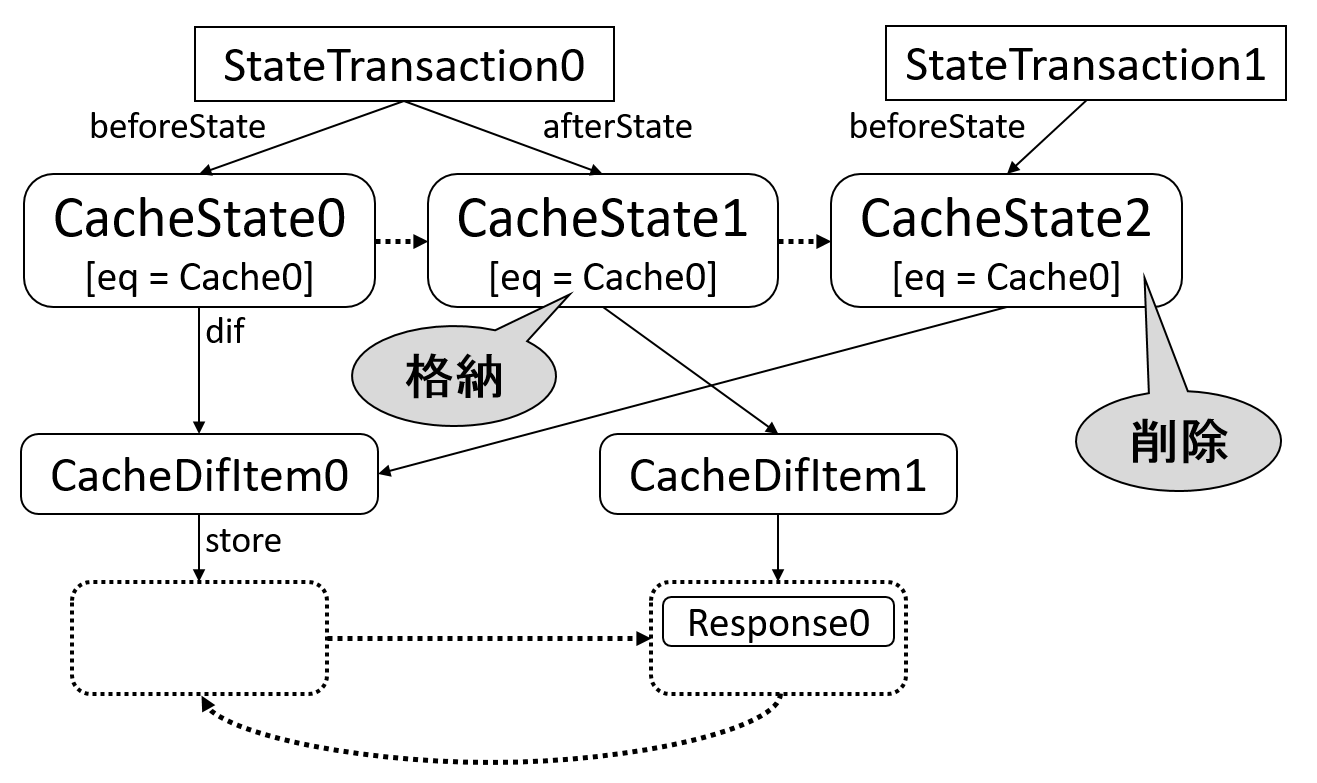
\includegraphics[width=450pt]{./fig/ProposedModel-ResponseStoreDelete.eps}
\caption{キャッシュの格納と削除の表現}
\label{fig:ProposedModel-ResponseStoreDelete}
\end{figure}

また,以上の内容を提案モデルではCode\ref{code:StoreResponse}のように実装している.
格納と削除は主に6-10行目で表されており,状態postがリクエスト時の状態である場合は,postの格納レスポンスの集合はpostの前状態であるpreの格納レスポンスの集合の部分集合となる.
この2状態の関係を部分集合とすることで,前状態の格納レスポンスの一部がなくなることを容認し,削除の動作を表現している.
また,状態postがレスポンス時の状態である場合は,上述の削除に加え,格納が行われている可能性がある.
したがって,postの格納レスポンスの集合を,preの格納レスポンスにそのトランザクションでのレスポンスを加えた和集合の部分集合とする.
これにより,削除に加え,レスポンス時における格納を表現している.
ただしこの記述のみでは各時点でのキャッシュの状態はその前状態に依存することになり,初期状態が無条件となる.
実際には,この場合の初期状態とはウェブ上における様々な通信が行われる前の状態を示すため,初期状態でキャッシュにレスポンスが格納されていることはない.
したがって,初期状態の格納レスポンスの集合を空集合とする制限を,2-4行目で記述している.

\begin{lstlisting}[caption=レスポンスの格納と削除の表現, label=code:StoreResponse]
fact flowCacheState{
	all cs:CacheState |
		InitialState[cs] implies
			no cs.dif.store

	all pre, post:CacheState, str:StateTransaction |
		LastState[pre, post, str] implies {
			post in str.beforeState implies post.dif.store in pre.dif.store
			post in str.afterState implies post.dif.store in (pre.dif.store + str.response)
		}
}
\end{lstlisting}

\subsubsection{レスポンスの再利用}
提案モデルにおいて,キャッシュによるレスポンスの再利用は以下の動作を示す.

\begin{itembox}[l]{レスポンスの再利用}
キャッシュは,そのキャッシュが存在する端末が送受信するリクエストに対して,キャッシュ内の格納レスポンスで応答できる場合,そのレスポンスを用いて応答することができる.
ここで,リクエストの送信者が自身のキャッシュで再利用を行う場合,リクエストは実際はネットワーク上に発信されない.
\end{itembox}

上記で定めたレスポンスの再利用は,提案モデル内では本来発生するレスポンスの代わりとなって発生する.
したがって,既存モデルにおいてレスポンスを表すHTTPResponseクラスと同列に,CacheReuseクラスを定義する(Code\ref{code:CacheReuseClass}参照).
HTTPResponseクラスはHTTPプロトコル上のイベントを表すHTTPEventクラスを継承しているため,CacheReuseクラスもHTTPEventクラスを継承する.
そして,CacheReuseクラスにある1つのレスポンスを関連付けることで,どのレスポンスを再利用したかを表現できる(5行目).
また,HTTPEventクラスにおいて,どの端末からどの端末に対するイベントであるかは定義されており,これを利用することで再利用したレスポンスの送信元と送信先を表現する.
しかし,HTTPEventクラスでは送信元と送信先の他に,そのイベントに含まれるヘッダとボディが定義されている.
実際のレスポンスの再利用では,送信されるのは再利用するレスポンスのヘッダとボディであり,それは上記のレスポンスとの関連付け(5行目)で表現されているためこの2項目は不必要である.
したがって,CacheReuseクラスとヘッダとボディの関係性は無視することができるが,ヘッダやボディを表すインスタンスは非常に多いため,無制限とした場合には無駄な計算時間を要することとなる.
このような要因から,7,8行目のようにCacheReuseクラスのヘッダとボディは空集合とし,計算時間の短縮を図る.

\begin{lstlisting}[caption=CacheReuseクラス, label=code:CacheReuseClass]
sig HTTPResponse extends HTTPEvent {
	statusCode: one Status
}
sig CacheReuse extends NetworkEvent{
	target: one HTTPResponse
}{
	no headers
	no body
}
\end{lstlisting}

上記で定義したCacheReuseクラスを用いて再利用を表現するため,Code\ref{code:happenCacheReuse}のように実際のキャッシュの動作に基づいた条件を付加する.
付加した条件は以下の通りである.
\begin{itemize}
\item 再利用レスポンスの送信先は,その再利用を発生させたリクエストの送信元である(5行目)
\item 再利用レスポンスの送信元は,その再利用を発生させたリクエストの送信元か送信先のいずれかである(6行目)
\item 再利用を行うキャッシュの再利用直前の状態において,再利用するレスポンスが格納レスポンスに含まれている(8-13行目)
\item 再利用するレスポンスと,その再利用を発生させたリクエストが表すURIが一致している(15行目)
\end{itemize}

\begin{lstlisting}[caption=CacheReuseの発生条件, label=code:happenCacheReuse]
fact happenCacheReuse{
	all reuse:CacheReuse | one str:StateTransaction |
		{
			str.re_res = reuse
			reuse.to = str.request.from
			reuse.from in str.request.(from + to)

			some pre, post:CacheState |
				(post in str.afterState and LastState[pre, post, str]) implies
					{
						reuse.target in pre.dif.store
						reuse.from.cache = pre.eq.cache
					}

			reuse.target.uri = str.request.uri
		}
}
\end{lstlisting}

上記の条件の2点目において,再利用レスポンスの送信元がリクエストの送信元となる場合を認めるのは,そのリクエストを送信した端末のキャッシュによるレスポンスの再利用を想定するためである.
例えば,図\ref{fig:BrowserCacheReuse}のようなブラウザキャッシュによるレスポンスの再利用である.
図\ref{fig:BrowserCacheReuse}はブラウザがサーバにリクエストを送信する際に,ブラウザのキャッシュ内に既に格納されているレスポンスResponse0を再利用する流れを表している.
このような場合には,CacheReuse0のfromとtoは同一のBrowser0を指すことになる.
2点目の条件は,このような状況を想定している.

\begin{figure}[htb]
\centering
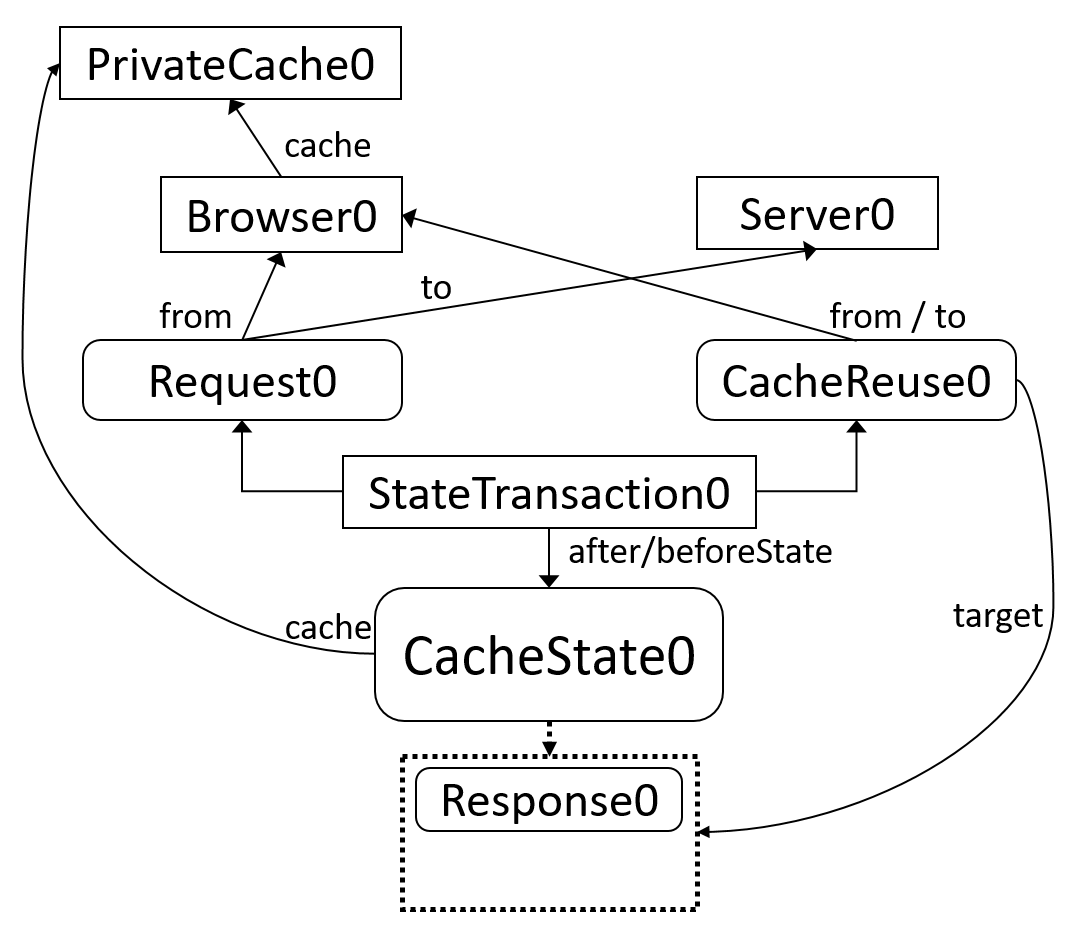
\includegraphics[width=350pt]{./fig/BrowserCacheReuse.eps}
\caption{ブラウザキャッシュでのレスポンスの再利用の一例}
\label{fig:BrowserCacheReuse}
\end{figure}

\subsubsection{格納レスポンスの検証}
\label{sec:CacheVerification}
提案モデルにおいて,キャッシュによる格納レスポンスの検証を以下のように定義する.

\begin{itembox}[l]{格納レスポンスの検証}
格納レスポンスは,格納レスポンスが再利用可能であるかを判定するために,条件付きリクエストを送信しオリジンサーバに問い合わせを行う.
条件付きリクエストは,if-modified-sinceヘッダかif-none-matchヘッダのいずれかが含まれるリクエストのことを指す.
これらのヘッダで送信される値を用いることで,オリジンサーバは格納レスポンスが最新のものと同一であるかを判定でき,再利用の可否をレスポンスで送信する.
検証が正常に終了した場合,このレスポンスの状態コードは304か200となる.
\begin{itemize}
\item 状態コードが304である場合 \\
そのヘッダやボディの値に関係なくキャッシュは格納レスポンスを再利用できる
\item 状態コードが200である場合 \\
格納レスポンスは再利用不可であり,このレスポンスをキャッシュに格納して再利用する
\end{itemize}
また,検証後はどちらの場合も再利用可能なレスポンスの1つを除いて,同一のURIに対するレスポンスはキャッシュ内には存在しない.
\end{itembox}

この動作の実装は以下の2つを表現することで実現できる.
\begin{itemize}
\item レスポンスの再利用が行われている場合に,その再利用レスポンスが検証済みであるかを判定する述語
\item 条件付きリクエストに対するサーバの動作
\end{itemize}

まず,検証済みかを判定する述語checkVerificationをCode\ref{code:checkVerification}に示す.
この述語checkVerificationはStateTransaction(strとする)を入力とする.
述語checkVerificationは,strが再利用によって応答されているトランザクションであり,かつ,strのリクエストと再利用の間に条件付きリクエストを含むトランザクションが成立している場合に真となるように作成し,その論理は以下のように表せる.

\begin{itembox}[l]{述語checkVerification}
入力であるStateTransactionクラスのインスタンスであるstrが再利用を行っており,かつ,以下を満たすStateTranactionのクラスのインスタンスstr'が存在する場合に,本述語は真となる.
\begin{itemize}
\item strとstr'は異なるトランザクションである(6行目)
\item str'のレスポンスが存在する.つまり,通信が正常に完了している(7行目)
\item str'のリクエストはstrの後に発生し,str'のレスポンスはstrの再利用より前に発生している(9,10行目)
\item str'のリクエストは,strの再利用が行われるキャッシュが属する端末から,再利用するレスポンスの送信元に送信されている(12,13行目)
\item strとstr'での要求URIが同一である(14行目)
\item 検証対象の格納レスポンスにetagヘッダかlast-modifiedヘッダが含まれている(16-19行目)
\item 検証対象の格納レスポンスにetagヘッダが含まれている場合,str'のリクエストにif-none-matchヘッダが含まれる(21,22行目)
\item 検証対象の格納レスポンスにlast-modifiedヘッダが含まれている場合,str'のリクエストにif-modified-sinceヘッダが含まれる(23,24行目)
\end{itemize}
\end{itembox}

\begin{lstlisting}[caption=ある再利用が検証済みか判定する述語, label=code:checkVerification]
pred checkVerification[str:StateTransaction]{
	one str.re_res

	some str':StateTransaction |
	{
		str' != str
		one str'.response

		str'.request.current in str.request.current.*next
		str.re_res.current in str'.response.current.*next

		str'.request.from = str.re_res.from
		str'.request.to = str.re_res.target.from
		str'.request.uri = str.request.uri

		some h:HTTPHeader |{
			h in ETagHeader + LastModifiedHeader
			h in str.re_res.target.headers
		}

		(some h:ETagHeader | h in str.re_res.headers) implies
			(some h:IfNoneMatchHeader | h in str'.request.headers)
		(some h:LastModifiedHeader | h in str.re_res.headers) implies
			(some h:IfModifiedSinceHeader | h in str'.request.headers)
	}
}
\end{lstlisting}

また,条件付きリクエストに関するサーバの動作をCode\ref{code:ConditionalRequestTransaction}に示す.
Code\ref{code:ConditionalRequestTransaction}内で,HTTPTransactionクラスのインスタンスtrが条件付きリクエストである場合,以下を満たす.
\begin{itemize}
\item 検証後に,その検証対象のレスポンスのURIを持つ格納レスポンスは1つとなる(5-14行目)
\item trのレスポンスの状態コードは200か304である(16行目)
\item trのレスポンスの状態コードが200である場合,trのレスポンスはキャッシュに格納される(18-23行目)
\item trのレスポンスの状態コードが304である場合,trのレスポンスはキャッシュに格納されない(25-30行目)
\end{itemize}

\begin{lstlisting}[caption=条件付きリクエストに対するサーバの動作, label=code:ConditionalRequestTransaction]
fact ConditionalRequestTransaction{
	all tr:HTTPTransaction |
		(some h:HTTPHeader | h in IfNoneMatchHeader + IfModifiedSinceHeader and h in tr.request.headers) implies
		{
			one res:HTTPResponse |
			{
				res.uri = tr.response.uri
				one cs:CacheState |
				{
					res in cs.dif.store
					cs.eq.cache = tr.request.from.cache
					cs in tr.afterState
				}
			}

			tr.response.statusCode in c200 + c304

			tr.response.statusCode = c200 implies
			{
				all cs:CacheState |
					(cs in tr.afterState and cs.eq.cache = tr.response.to.cache) implies
						tr.response in cs.dif.store
			}

			tr.response.statusCode = c304 implies
			{
				all cs:CacheState |
					(cs in tr.afterState and cs.eq.cache = tr.response.to.cache) implies
						tr.response !in cs.dif.store
			}
		}
}
\end{lstlisting}

\section{中継者の実装}
提案モデルにおいて中継者はHTTP/HTTPSプロトコルで動作し,プロキシとゲートウェイを包括する.
したがって,HTTPに遵守する端末を表すHTTPConfirmistを継承する形で中継者のクラスを宣言する.
また,中継者のクラスを継承し,プロキシとゲートウェイのクラスを宣言する.
これらのクラスは以下のコードで実装される.

\begin{lstlisting}[caption=中継者,プロキシ,ゲートウェイのクラス, label=code:IntermediaryClass]
abstract sig NetworkEndpoint{}
abstract sig HTTPConformist extends NetworkEndpoint{cache : lone Cache}
abstract sig HTTPIntermediary extends HTTPConformist{}
sig HTTPProxy extends HTTPIntermediary{}
sig HTTPGateway extends HTTPIntermediary{}
\end{lstlisting}

基礎モデルの要素も含め,提案モデルでのネットワーク構成要素のクラス関係は図\ref{fig:NetworkComponent}のようになる.

\begin{figure}[htb]
\centering
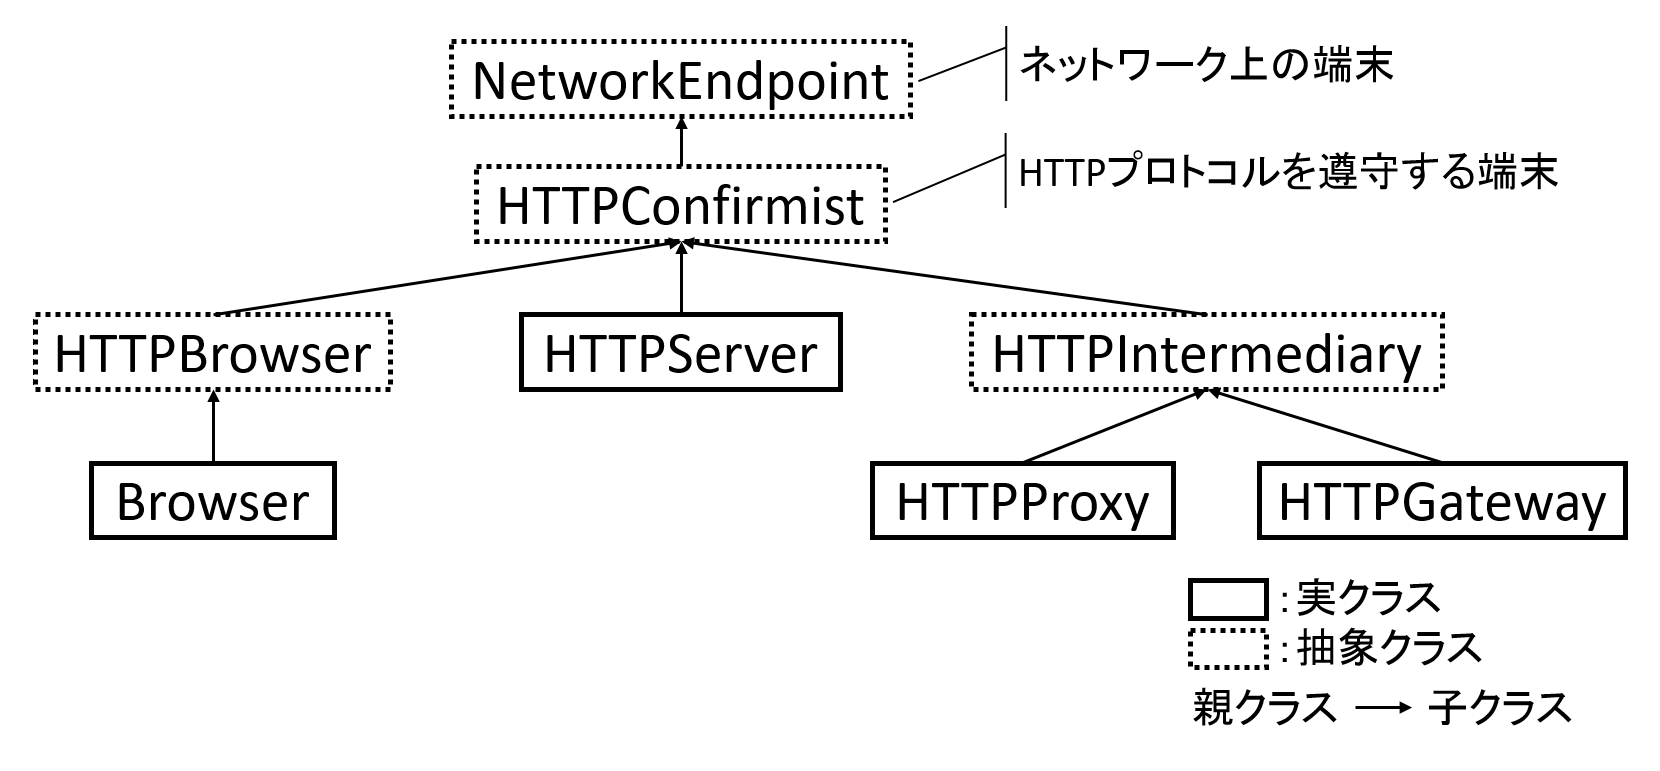
\includegraphics[width=450pt]{./fig/NetworkComponent.eps}
\caption{提案モデルにおけるネットワーク構成要素のクラス関係}
\label{fig:NetworkComponent}
\end{figure}

また,この中継者の動作をCode\ref{code:MoveOfIntermediary}のように記述する.
中継者の動作はリクエストの送信先がHTTPIntermediaryであり,かつ,レスポンスが存在するHTTPTransactionに対する条件として記述する.
このようなHTTPTransactionのインスタンスtrに対して,以下を満たすHTTPTransactionのインスタンスtr'が少なくとも1つ存在する.
\begin{itemize}
\item trとtr'は異なるトランザクションである(5行目)
\item tr'のリクエストはtrのリクエストの後に発生し,tr'のレスポンスはtrのレスポンスの前に発生する(7,8行目)
\item tr'のリクエストの送信元は,trのリクエストの送信先である中継者である(9行目)
\item trとtr'のリクエストのURIは同一である(12行目)
\item trとtr'のレスポンスのbodyと状態コードは同一である(13,14行目)
\end{itemize}
ただし,上記の動作は正当なユーザに管理された中継者の動作であり,攻撃者が管理する中継者のふるまいはこの限りではない.

\begin{lstlisting}[caption=中継者の動作, label=code:MoveOfIntermediary]
fact MoveOfIntermediary{
	all tr:HTTPTransaction |{
		tr.request.to in HTTPIntermediary and one tr.response implies{
			some tr':HTTPTransaction |{
				tr != tr'				
				
				tr'.request.current in tr.request.current.*next
				tr.response.current in tr'.response.current.*next

				tr.request.to in WebPrincipal.servers implies{
					tr'.request.from = tr.request.to
					tr'.request.uri = tr.request.uri
					tr.response.body = tr'.response.body
					tr.response.statusCode = tr'.response.statusCode
				}
			}
		}
	}
}
\end{lstlisting}

%\section{提案モデルの制限事項}

\end{document}

\documentclass[12pt,a4paper]{jbook}
\usepackage{mm-thesis}
\usepackage[dvipdfmx]{graphicx}
\usepackage{cite}
\usepackage{comment}
\usepackage{docmute}
\usepackage{color}
%\usepackage{amsmath}
%\usepackage{amsthm}
%\usepackage{amsfonts}

\begin{document}
\newpage

\chapter{事例研究}
本章では、複数の具体的な事例を取り上げ、提案モデルの実装の正しさを確認する。

\section{キャッシュの基本動作}
本節では、提案モデルでのキャッシュの実装の正しさを確認する。
提案モデルにおいて、キャッシュは主に格納、再利用、検証の三つの動作を行う。
それぞれについて、実行ツールAlloy Analyzerの実行結果を確認する。

\subsection{レスポンスの格納}
レスポンスの格納動作を確認するため、実行結果からレスポンスの格納を伴う動作を抽出する。
ここでは簡単のため、最も単純な二者間における通信で生じるレスポンスの格納を対象とし、Code\ref{code:test_store}を用いて実行結果を出力を得る。

\begin{lstlisting}[caption=レスポンスの格納, label=code:test_store]
run test_store{
	#HTTPClient = 1
	#HTTPServer = 1
	#HTTPRequest = 1
	#HTTPResponse = 1
	some CacheState.dif.store
} for 2
\end{lstlisting}

得られる出力結果を整理し、図\ref{fig:TestStore}に示す。
図\ref{fig:TestStore}には、PrivateCache0を持つBrowser0とServer0間の、Request0とResponse0のトランザクションにおけるキャッシュの状態変化が示されている。
最初、リクエスト時にはキャッシュの状態はCacheState0で示されており、CacheState0の変化要素を表すCacheDifItem0のstoreが空集合である。
しかし、レスポンス時には状態はCacheState1に変化しており、対応するCacheDifItem1がResponse0にstoreを指している。
以上より、図\ref{fig:TestStore}はあるトランザクションにおいて、レスポンスがブラウザキャッシュに格納されている状態を表しており、レスポンスの格納が表現可能であることが確認できる。

\begin{figure}[htb]
\centering
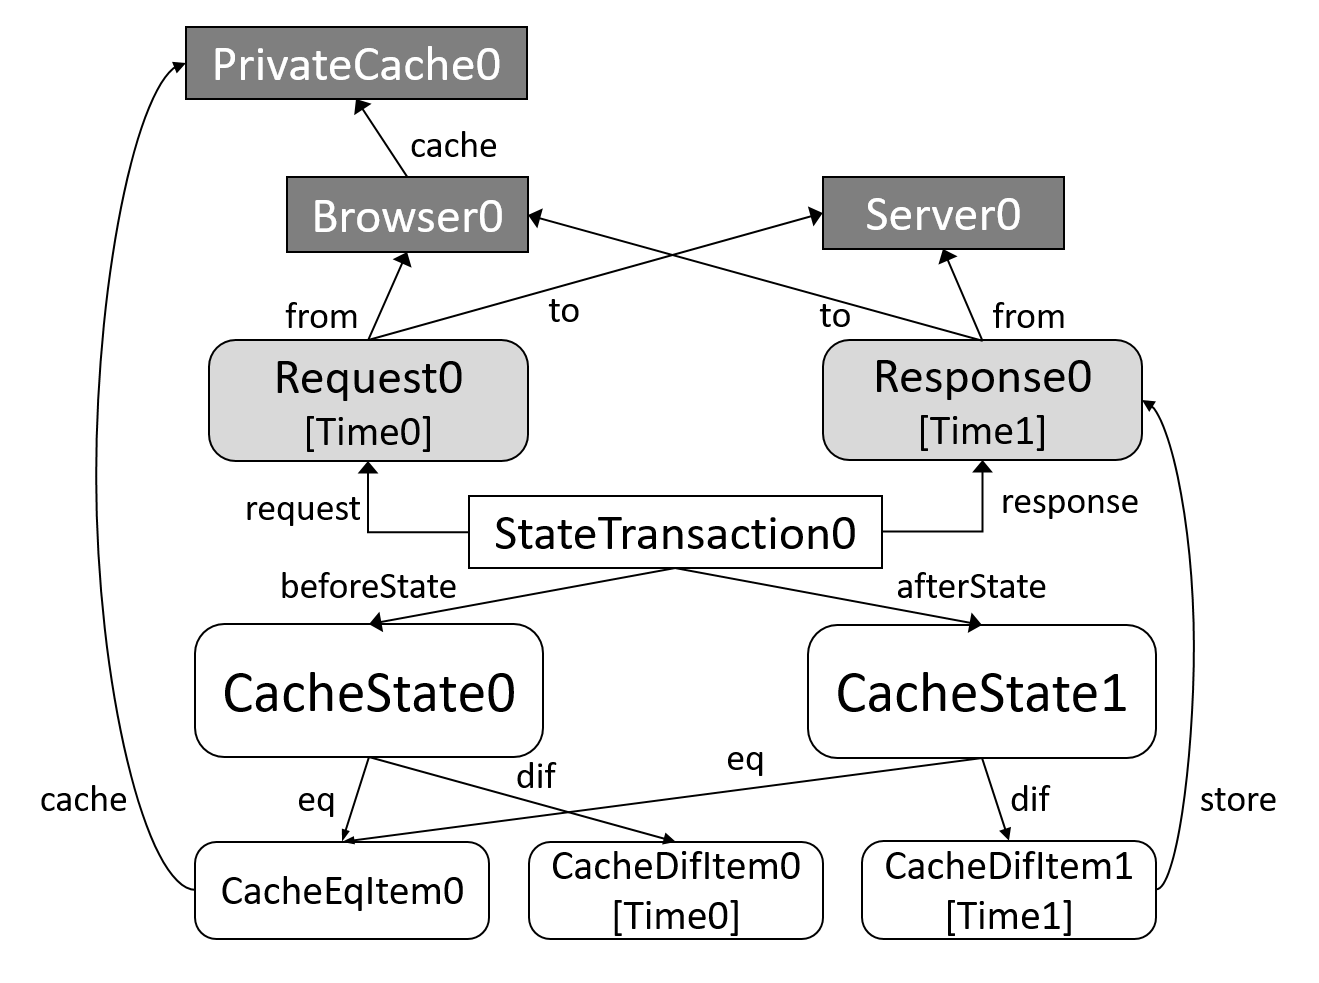
\includegraphics[width=450pt]{./fig/TestStore.eps}
\caption{レスポンスを格納する状態の一例}
\label{fig:TestStore}
\end{figure}

\subsection{レスポンスの再利用}
レスポンスの再利用動作を確認するため、実行結果からレスポンスの再利用を伴う動作を抽出する。
ここでは簡単のため、最も単純な二者間における通信で生じるレスポンスの再利用を対象とし、Code\ref{code:test_reuse}を用いて実行結果を出力を得る。

\begin{lstlisting}[caption=レスポンスの再利用, label=code:test_reuse]
run test_reuse{
	#HTTPClient = 1
	#HTTPServer = 1
	#Cache = 1

	#HTTPRequest = 2
	#HTTPResponse = 1
	#CacheReuse = 1
} for 4
\end{lstlisting}

得られる出力結果をスペースの都合上一部簡略化し、図\ref{fig:TestReuse}に示す。
図\ref{fig:TestReuse}はあるキャッシュを持つブラウザとサーバ間で、同様のURIに対してリクエストが二回送信された状態を表している。
ここで、StateTransaction0は図\ref{fig:TestStore}と同様、ブラウザキャッシュにResponse0を格納していることを示している。
StateTransaction1では、この格納レスポンスを再利用するイベントCacheReuse0が発生している。
以上より、図\ref{fig:TestReuse}に示す出力結果から、再利用を伴う動作が表現可能であることが確認できる。

\begin{figure}[htb]
\centering
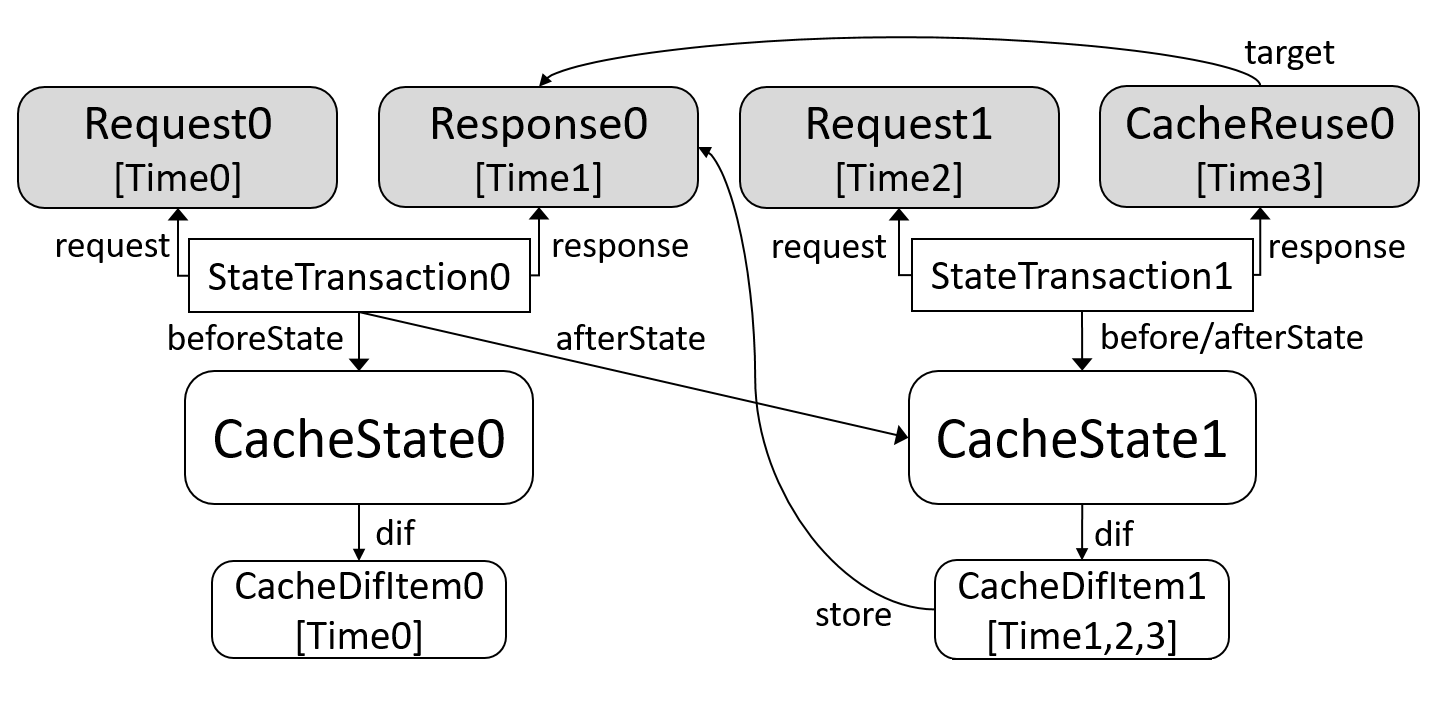
\includegraphics[width=450pt]{./fig/TestReuse.eps}
\caption{格納レスポンスを再利用する状態の一例}
\label{fig:TestReuse}
\end{figure}

\subsection{レスポンスの検証}

\section{中継者の基本動作}

\section{Browser Cache Poisoning Same-origin Attack}

\section{Browser Cache Poisoning Cross-origin Attack}

\section{Web Cache Deception Attack}

\section{Cross-site Request Forgeries Attack}

\end{document}

\documentclass[12pt,a4paper]{jbook}
\usepackage{mm-thesis}
\usepackage[dvipdfmx]{graphicx}
\usepackage{cite}
\usepackage{comment}
\usepackage{docmute}
\usepackage{color}
%\usepackage{amsmath}
%\usepackage{amsthm}
%\usepackage{amsfonts}

\begin{document}
\newpage

\chapter{おわりに}
本研究では,ウェブの安全性解析に形式手法を用いることを目的とし,ウェブを構成する要素の状態変化を表現するための時相論理を,Alloy上で表現するための記述法を考案した.
また,この記述法を用いてキャッシュを表現したウェブセキュリティモデルを実装し,その表現能力を評価した.

提案記述法では,様々なウェブの構成要素の状態を表現可能な汎用的なクラスを定義した.
また,このクラスのインスタンスを時系列順に並び替えるために利用できる2つの述語を実装した.
これにより,ウェブに含まれる要素の時系列順の状態変化を表現することが可能となる.

また,この記述法を用いてキャッシュを実装したウェブセキュリティモデルでは,実際にキャッシュの基本的な動作を表現できることを確認した.
これに加えて,既存のウェブセキュリティモデルでは表現できなかった状態遷移を含む四つの攻撃法について表現可能であることを確認し,モデルの表現能力の向上を達成した.
本研究では,これらの攻撃法のモデルによる表現を実現したが,対策法の考案には至っていない.
ここで得られた出力結果を元に,攻撃法が成功しない条件の発見が今後の課題である.

また一方で,本研究で実装した提案モデルではHTTPSの拡張プロトコルであるHTTP Strict Transport Security\cite{hsts},Public Key Pinning Extension for HTTP\cite{hpkp}に対する応用も課題である.
これらは現在ウェブでの実用化がすすめられているプロトコルであり,安全性解析を要するものであるが,プロトコルの操作に必要なヘッダが提案モデルに不足しているため,提案モデルでの安全性解析が不可能である.
しかし,これらのプロトコルがキャッシュを用いてHTTPSの安全性を向上させたものであるため,提案モデルの拡張によるこれらのプロトコルの表現は現実的であると考えている.

\end{document}


\acknowledgement
まず,本研究を進める全過程において多大な御指導を賜りました藤原融教授に深く感謝致します.
また,矢内直人助教,岡村真吾招聘准教授に心より御礼申し上げます.
そして,日常の議論を通じて多くのアドバイスや指摘を下さった藤原研究室の皆様ならびに,円滑な研究生活のために諸事務手続きを行って下さった秘書の方々に感謝致します.

\bibliographystyle{junsrt}
\bibliography{list} 

\end{document}


